\documentclass[12pt,titlepage]{article}

\usepackage{amsmath,amsthm}
\usepackage{unicode-math}
\usepackage{xltxtra}
\usepackage{xgreek}

\setmainfont{Times New Roman}

\usepackage{tabularx}

\usepackage[table]{xcolor}
\usepackage{tikz}
\pagestyle{empty}

\usepackage{geometry}
 \geometry{a4paper, top=53mm, bottom=53mm, left=40mm, top=40mm}

 \usepackage{graphicx}


 \usepackage{wrapfig}

 \renewcommand{\baselinestretch}{1.5}

 \newtheorem{proposition}{Πρόταση}
 \newtheorem{corollary}{Πόρισμα}


%% \usepackage{hyperref}
%%\address{Ερυθραίας 46\\ 54351 Θεσσαλονίκη}

\begin{document}

\begin{titlepage}
 \begin{center}
  \Huge {Η συνάρτηση $\ln x$ ως εμβαδό}

  \vspace{1.5cm}
  \Large {Μαθηματικά και οι άλλες επιστήμες στην εκπαίδευση}
 \end{center}

 \vspace{2cm}
 \begin{center}

  \begin{tabular}{ c c }
   \Large{Κωνσταντίνος} & \Large{Παγώνα}\\
   \Large{Λόλας} & \Large{Παπακωνσταντίνου} \\
   \textit{Γραβιάς 15,} & \textit{Γραβιάς 15,} \\
   \textit{Θεσσαλονίκη} & \textit{Θεσσαλονίκη} \\
   τηλ.6973380837 & τηλ.6958386849\\
   costasmath@yahoo.gr & pecoaganzi@gmail.com \\
  \end{tabular}

  \vspace{2cm}
  \textbf{Περίληψη}

  Γνωρίζουμε φυσικά ότι $\int_1^t \frac{1}{x}=\ln t$. Οι μαθητές όμως της Β Λυκείου στη Φυσική Κατεύθυνσης μαθαίνουν ότι το έργο που παράγεται ή καταναλώνεται αντιστοιχεί στο εμβαδό μεταξύ της γραφικής παράστασης της συνάρτησης $P=P(V)$ του άξονα $V$ και μεταξύ δύο όγκων $V_a$ και $V_b$. Έτσι αφού ο τύπος (καταστατική εξίσωση) για τα ιδανικά αέρια είναι ο $PV=nRT$, για να βρεθεί το έργο σε μία ισόθερμη μεταβολή ζητάται το εμβαδό μεταξύ της $P(V) = nRT\frac{1}{V}$ με $n$, $R$ και $T$ σταθερά, του άξονα των $V$ και μεταξύ δύο όγκων $V_a$ και $V_b$. Ο τύπος τους δίνεται χωρίς απόδειξη και ίσος με $W=nRT \ln \frac{V_b}{V_a}$ χωρίς να γνωρίζουν πώς το $\frac{1}{V}$ μετατρέπεται σε $\ln V$. Θα δείξουμε ότι υπάρχει συνάρτηση $f(x)$ που έχει τις ίδιες ακριβώς ιδιότητες με την συνάρτηση $\ln x$ και μάλιστα $f(a^x)=x$ με $a=e$. Συνεπώς $f(x)=\ln x$.

 \end{center}

\end{titlepage}

\section{Ορισμός της $f$}
Η συνάρτηση $f(t)$ ορίζεται ως το εμβαδό μεταξύ της συνάρτησης $\frac{1}{x}$ του άξονα των $x$ και των ευθειών $x=1$ και $x=t$. Χάριν συντομίας θα συμβολίζουμε το εν λόγω εμβαδό με $E_1^t$.

Θα αποδείξουμε για κάθε $x\in \mathbb{Q}$ ότι
$$f(e^x)=x$$
το οποίο σημαίνει ότι η $f$ είναι η αντίστροφη της $e^x$ δηλαδή η $\ln x$.

Για να φτάσουμε σε αυτή τη σχέση θα χρειαστούμε τις ιδιότητες:
\begin{enumerate}
  \item $f(e)=1$
  \item $f(a^k)=kf(a)$, $k\in \mathbb{Q}$
  \item $f(a^k)=kf(a)$, $k\in \mathbb{N}$
  \item υπάρχει $a$ ώστε $f(a)=1$
  \item $f(ab)=f(a)+f(b)$
\end{enumerate}

\section{Ιδιότητα $f(ab)=f(a)+f(b)$}
Πρώτα θα αποδείξουμε ότι $E_a^{ab}=E_1^b$. Γραφικά και για $b=2$:
\begin{figure}[h]
 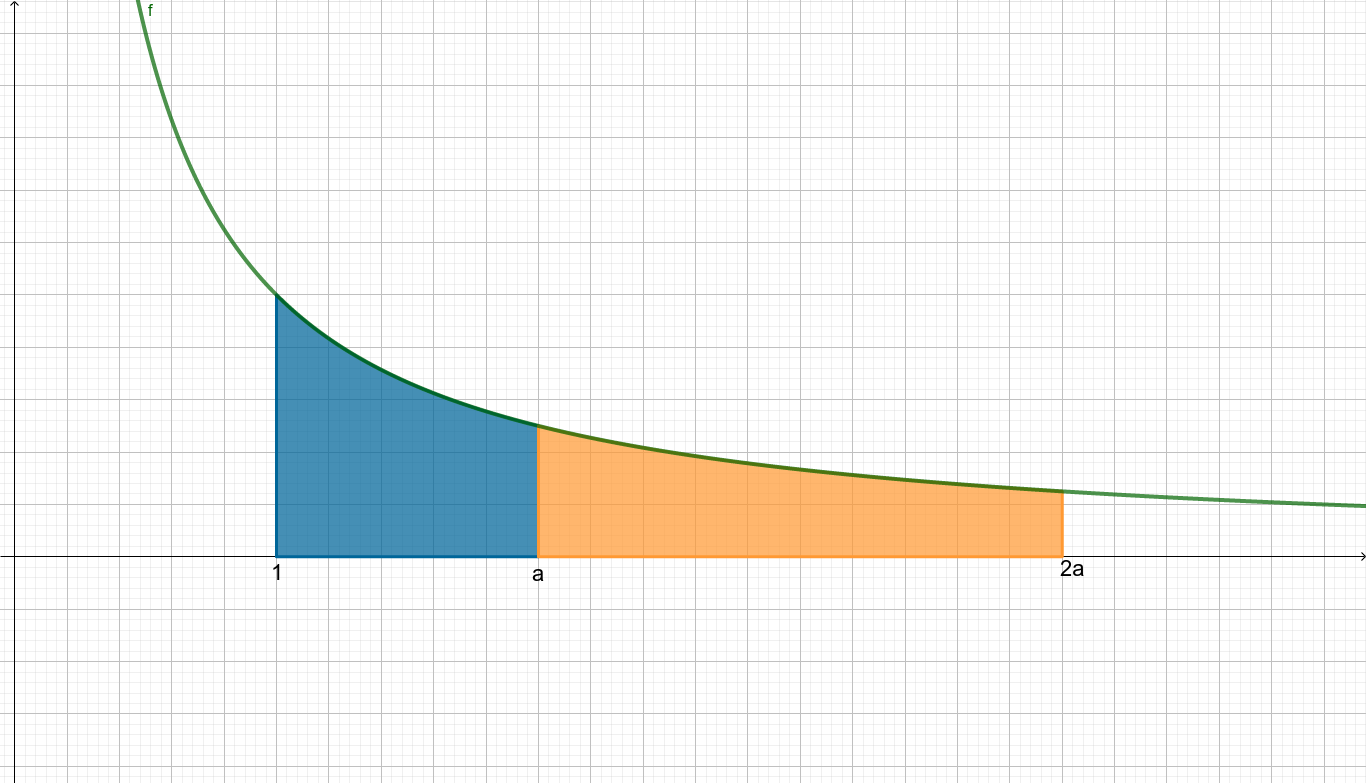
\includegraphics[width=0.6\textwidth]{1overX.png}
 \centering
\end{figure}
Τα δύο γραμμοσκιασμένα σχήματα έχουν το ίδιο ακριβώς εμβαδό. Αν "τεντώσουμε" (ή συρικνώσουμε) το μήκος κατά $a$ και "συρικνώσουμε" (αντ. τεντώσουμε) το πλάτος κατά $a$, τα εμβαδά θα ισούνται. Το ίδιο αποτέλεσμα επαληθεύεται και με την άλγεβρα της Β Λυκείου, στο κεφάλαιο 2.4 παράδειγμα 2ο. Αν έχουμε μία γραφική παράσταση μίας συνάρτησης $g(x)$ τότε η $g(ax)$ είναι μία μεγέθυνση αν $a>1$ (αντ. σμίκρινση αν $a<1$) στον άξονα των $x$ ενώ η $ag(x)$ είναι και πάλι μεγέθυνση αν $a>1$ (αντ. σμίκρινση αν $a<1$) αλλά αυτή τη φορά στον άξονα των $y$. Η συνάρτηση που έχουμε είναι η $g(x)=\frac{1}{x}$ για την οποία προφανώς ισχύει $ag(ax)=a\frac{1}{ax}=\frac{1}{x}=g(x)$. Δηλαδή αν μεγενθύνουμε στον άξονα $x$ και συρικνώσουμε ταυτόχρονα στον $y$ κατά κλίμακα $a$ βρίσκουμε την ίδια συνάρτηση, δηλαδή το ίδιο εμβαδό. Συνεπώς:
$$E_a^{ab}=E_1^{b}=E_1^b$$
Αλλά $E_a^{ab}=7f(ab)-f(a)$ και $E_1^b=f(b)$. Έτσι
$$f(ab)-f(a)=f(b) \Rightarrow f(ab)=f(a)+f(b)$$

\section{Ιδιότητα $f(1)=0$}
Προφανώς το εμβαδό $E_1^1=0$ και άρα $f(1)=0$.

\section{Ιδιότητα $f(\infty)=\infty$}
Αν χωρίσουμε το εμβαδό στα τμήματα
$$(1,b)\cup (b,2b) \cup (2b,4b) \cup \cdots$$
τότε το συνολικό εμβαδό θα είναι $f(\infty)=f(b)+f(b)+f(b)+\cdots=\infty$.

\section{Ιδιότητα $f(a)=1$}
Αφού το εμβαδό στο $1$ είναι $0$ και σύμφωνα με την προηγούμενη ιδιότητα δεν είναι φραγμένο προς τα δεξιά, θα υπάρχει τιμή στην οποία θα ισούται με $1$. Έτσι υπάρχει $a>1$ ώστε $f(a)=1$.

\section{Ιδιότητα $f(\frac{1}{x})=-f(x)$}
Για τον ίδιο λόγο με την 1η ιδιότητα. Το σημείο $1/x$ βρίσκεται αριστερά από το $1$ και μάλιστα το διάστημα $(\frac{1}{x},1)$ είναι σμίκρυνση του διαστήματος $(1,x)$ κατά $x$ στον οριζόντιο άξονα. Το πρόσημο $-$ μπροστά στο $f(x)$ έχει να κάνει με τη σύμβαση ότι θα θεωρούμε κάθε εμβαδό προς τα δεξιά θετικό, ενώ προς τα αριστερά αρνητικό.

\section{Ιδιότητα $f(a^k)=k$, $k \in \mathbb{N}$}
Αν χωρίσουμε τα εμβαδά κάτω από την γραφική παράσταση στα διαστήματα
$$(1,a^k)=(1,a)\cup (a,a^2) \cup (a^2,a^3) \cup \cdots \cup (a^{k-1},a^k)$$
τότε τα εμβαδά θα ισούνται με
$$f(a^k)=f(a)+f(a)+f(a)+\cdots+f(a)=kf(a)$$

\section{Ιδιότητα $f(a^k)=k$, $k \in \mathbb{Q}$, $k>0$}
Έστω $k=\frac{m}{n}$. Τότε σύμφωνα με την προηγούμενη ιδιότητα
$$f(a^{\frac{m}{n}})=mf(a^\frac{1}{n})$$
Αν τώρα χωρίζουμε το διάστημα $(1,a)$ σε διαστήματα
$$(1,a)=(1,a^{\frac{1}{n}})\cup (a^{\frac{1}{n}},a^{\frac{2}{n}})\cup (a^{\frac{2}{n}},a^{\frac{3}{n}})\cup \cdots \cup (a^{\frac{n-1}{n}},a)$$
τότε και σύμφωνα με την πρώτη ιδιότητα θα ισχύει
$$f(a)=f(a^{\frac{1}{n}})+f(a^{\frac{1}{n}})+f(a^{\frac{1}{n}})+\cdots+f(a^{\frac{1}{n}})=nf(a^{\frac{1}{n}})$$
Δηλαδή
$$f(a^{\frac{1}{n}})=\frac{1}{n}f(a)$$
Αντικαθιστώντας στην αρχική σχέση
$$f(a^k)=f(a^{\frac{m}{n}})=mf(a^\frac{1}{n})=\frac{m}{n}f(a)=kf(a)$$

\section{Απόδειξη ότι $a=e$}
Το $E_1^{1+x}$ για πολύ μικρό $x\in \mathbb{Q}$ προσεγγίζει το ορθογώνιο με ύψος $1$ και μήκος $x$. Έτσι για $x\to 0$ ισχύει
$$f(1+x)=x \Rightarrow \frac{1}{x}f(1+x)=1 \Rightarrow f\left( (1+x)^{\frac{1}{x}} \right)=1$$
Το οποίο $(1+x)^{\frac{1}{x}}$ για $x\to 0$ ισούται με $e$. Δηλαδή $a=e$.

Δείξαμε λοιπόν ότι σε όλους τους ρητούς αριθμούς η $f$ έχει όλες τις ιδιότητες της συνάρτησης $\ln $.

Όλα τα προηγούμενα θα μπορούσαμε βέβαια να τα δείξουμε με την βοήθεια της άλγεβρας ή της ανάλυσης, αλλά σκοπός ήταν να γίνει μία προσέγγιση από την πλευρά της γεωμετρίας - εμβαδών. φ

\begin{thebibliography}{9}
άλγεβρα Β Λυκείου...

\end{thebibliography}
\end{document}
